\documentclass{cmc}

\begin{document}

\pagestyle{fancy}
\lhead{\textit{\textbf{Computational Motor Control, Spring 2020} \\
    Python exercise, Lab 5, GRADED}} \rhead{Zhou Xiao \\ Lu Xiaolong \\ Joseph Al Aaraj}

\section*{Student names: Zhou Xiao, Lu Xiaolong, Joseph Al Aaraj}
\textit{Instructions: Update this file (or recreate a similar one,
  e.g.\ in Word) to prepare your answers to the questions. Feel free
  to add text, equations and figures as needed. Hand-written notes,
  e.g.\ for the development of equations, can also be included e.g.\
  as pictures (from your cell phone or from a scanner).
  \textbf{\corr{This lab is graded.}} and must be submitted before
  the \textbf{\corr{Deadline : 22-04-2020 23:59}}.  \\ Please
  submit both the source file (*.doc/*.tex) and a pdf of your
  document, as well as all the used and updated Python functions in a
  single zipped file called \corr{lab5\_name1\_name2\_name3.zip} where
  name\# are the team member’s last names.  \corr{Please submit only
    one report per team!}}
\\

\textit{The file \fileref{lab\#.py} is provided to run all exercises
  in Python.
  % Each \fileref{exercise\#.py} can be run to run an exercise
  % individually.
  % The list of exercises and their dependencies are shown in
  % Figure~\ref{fig:files}.
  When a file is run, message logs will be printed to indicate
  information such as what is currently being run and and what is left
  to be implemented. All warning messages are only present to guide
  you in the implementation, and can be deleted whenever the
  corresponding code has been implemented correctly.}


\begin{figure}[ht]
  \centering 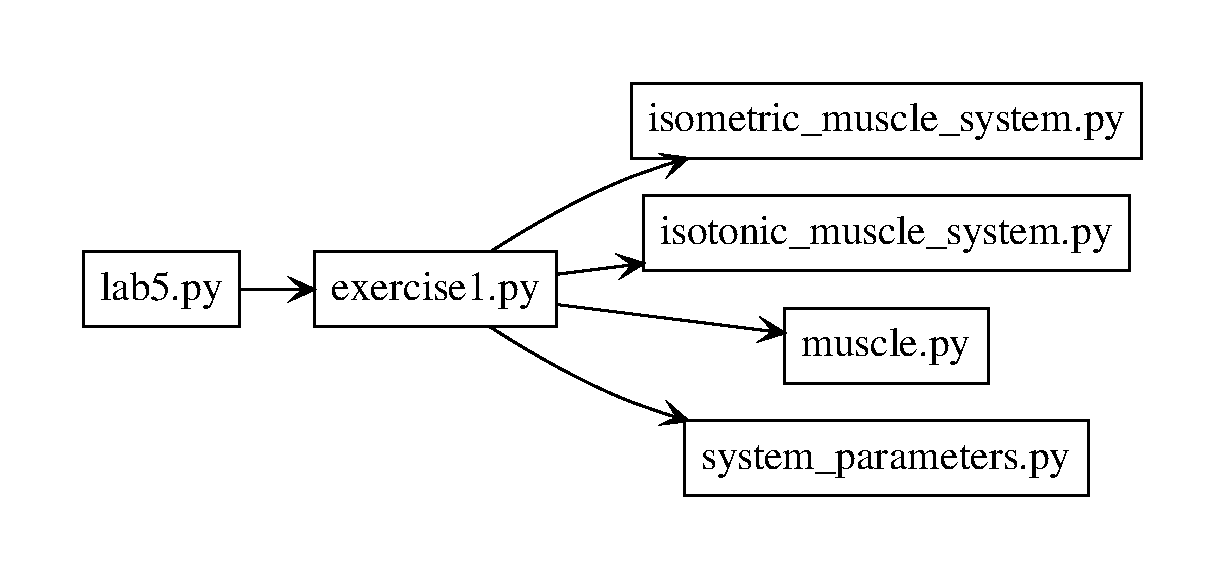
\includegraphics[width=0.5\textwidth]{figures/files}
  \caption{\label{fig:files} Exercise files dependencies. In this
  lab, you will be modifying \fileref{exercise1.py}.}
\end{figure}

\subsection*{Files to complete the exercises}
\label{sec:intro}

\begin{itemize}
\item \fileref{lab5.py} : Main file
\item \fileref{exercise1.py} : Main file to complete exercise 1
\item \fileref{system\_parameters.py} : Parameter class for Pendulum,
  Muscles and Neural Network (Create an instance and change properties
  using the instance. You do not have to modify the file)
\item \fileref{isometric\_muscle\_system.py} : Class to setup your isometric
  muscle test experiments (You do not have to modify the file)
\item \fileref{isotonic\_muscle\_system.py} : Class to setup your isotonic
  muscle test experiments (You do not have to modify the file)
\item \fileref{muscle.py} : Muscle class (You do not have to modify
  the file)
\item \fileref{mass.py} : Mass model class (You do not have to modify
  the file)
\end{itemize}

\textbf{NOTE : } '\textit{You do not have to modify}' does not mean
you should not, it means it is not necessary to complete the
exercises. But, \corr{you are expected to look into each of these
  files and understand how everything works}. You are free to explore
and change any file if you feel so.


\section*{Exercise 1 : Hill muscle model}
\label{sec:question-2}

Previous week you explored the role of different passive components
and the effects of its parameters on the system. In this exercise, we
try to understand the contractile or the active element of the hill
muscle model. The components of the hill muscle are described in
figure \ref{fig:hill_muscle}. The equations used to model the hill
muscle can be found in the pdf \fileref{HillMuscleEquations.pdf}

\begin{figure}[H]
  \centering 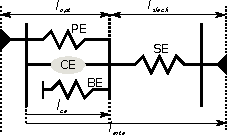
\includegraphics[scale=2.5]{figures/hill_muscle}
  \caption{Hill muscle model}
  \label{fig:hill_muscle}
\end{figure}

Where,

\begin{itemize}
\item $PE$ : Parallel element (Prevents muscle from over stretching)
\item $BE$ : Muscle Belly (Prevents muscle from collapsing on itself)
\item $SE$ : Series element or the muscle tendon element
\item $CE$ : Contractile Element or the active element
\item $l_{opt}$ : Muscle optimal fiber length
\item $l_{slack}$ : Muscle tendon slack length
\item $l_{ce}$ : Contractile element length
\item $l_{mtu}$ : Muscle Tendon Unit length
\end{itemize}


\begin{figure}[H]
  \centering
  \begin{subfigure}[b]{0.49\textwidth}
    { \centering
      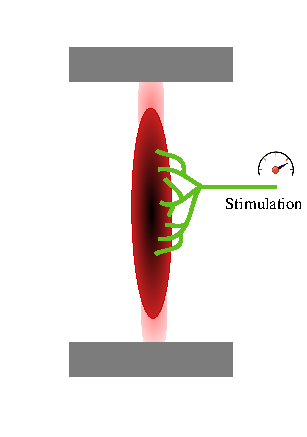
\includegraphics[width=\textwidth]{figures/isometric_muscle} }
    \caption{Isometric muscle setup :\\ To study the relationship
      between Force-Length.}
    \label{fig:isometric_muscle}
  \end{subfigure}
  \begin{subfigure}[b]{0.49\textwidth}
    { \centering
      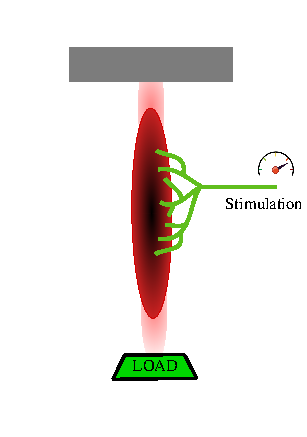
\includegraphics[width=\textwidth]{figures/isotonic_muscle} }
    \caption{Isotonic muscle setup :\\ To study the relationship
      between Force-Velocity.}
    \label{fig:isotonic_muscle}
  \end{subfigure}
  \caption{Muscle Length-Velocity-Force Setup}
  \label{fig:muscle-setup}
\end{figure}

\subsection*{Muscle Force-Length Relationship}
\label{sec:muscle-force-length}
In this exercise you will explore the relation between the length and
velocity of the muscle. In order to do this we replicate the set-up
show in figure \ref{fig:muscle-setup}.Here the length of the muscle is
held constant by attaching it's tendon to two fixed points. While
applying a constant stimulation, observing the force produced will
give the relationship between muscle contractile element length and
force.
\subsection*{1.a For a given stimulation, explore the relationship
  between active and passive muscle forces and the length of the
  contractile element.  Plot the force-length relationship curve.
  Discuss the different regions in the plot. Use the
  \fileref{isometric\_muscle\_system.py::IsometricMuscleSystem} instance
  to setup your experiment in \fileref{exercise1.py}}


Forces in muscles is dependent of contractile proteins: myosin and actin filaments bounded by thin Z disks in the sarcomeres, which are distributed in series inside the myofibrils. (P1,P2) When the muscle is activated,contraction is produced by cyclical attachments of myosin heads to the actin.

\begin{figure}[H]
  \centering 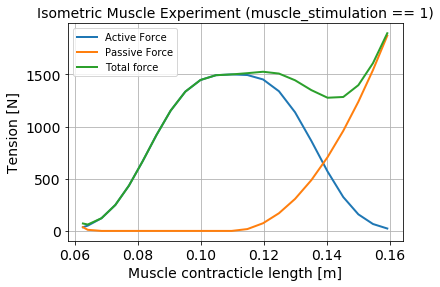
\includegraphics[height=7cm]{Lab5/Report/figures/1a.png}
  \caption{Relationship between forces and contractile element length in isometric muscle experiment}
  \label{1a}
\end{figure}

In this isometric case, the curves for active force, passive force and the total force, as a function of muscle elongation can be observed from Figure 4.
The active contractile force developed during contraction depends on the degree of overlap of thick and thin filaments. 
It can depends on the external input signals (neuron). When the muscle is too short, this force can not be generated.
Exceeding a certain length, as the muscle elongates,the active force increase. The increase rate decreases until it reaches a maximum at optimal length, and then it decreases.
When the elongation is too long, the overlap of thick (myosin) and thin (actin) filaments is too short to generate the contractile force and it can develop to very low value.
On the other hand, the passive force, which is resistant to further elongating, will be generated once the elongation of muscle exceeds a certain length. It increases almost exponentially as the muscle elongates before arriving a certain limit. This force is the intrinsic property of the muscle, and it can not be modified because it depends on its physical structure and composition.
Finally, the total force is the plus of active and passive force. 


\subsection*{1.b In (1.a), you explored the muscle force-length
  relationship for a given stimulation. What happens to the
  relationship when the stimulation is varied between [0 - 1]? Support
  your response with one plot showing the different force-length
  relationship curves.}
  \begin{figure}[H]
  \centering 
  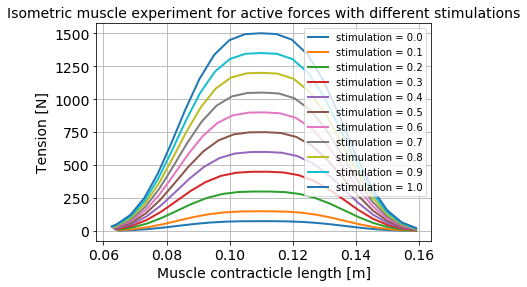
\includegraphics[height=0.3\columnwidth]{Lab5/Report/figures/1b_active.png}
  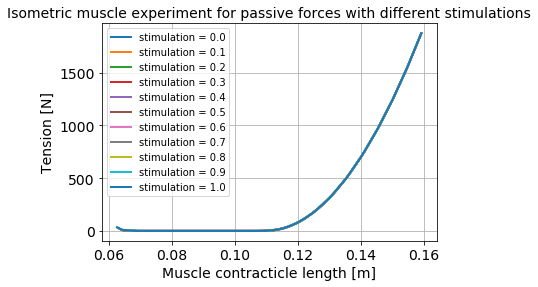
\includegraphics[height=0.3\columnwidth]{Lab5/Report/figures/1b_passive.png}
  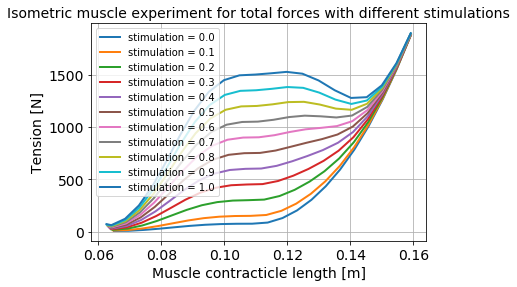
\includegraphics[height=0.3\columnwidth]{Lab5/Report/figures/1b_total.png}
  \caption{Relationship between forces and contractile element length with different stimulations in isometric muscle experiment }
  \label{1b}
\end{figure}
  
As can be seen from the above plots in Figure 5, an increase in stimulation causes an increase in the active forces, yet passive forces remain constant. What is noteworthy at first is fact that no matter how much the stimulation is increased or decreased, the muscle stretch always remain the same. Second, passive forces of a muscle are intrinsic properties of that muscle. Electric stimulation does not affect any intrinsic properties, and hence, passive forces remain constant. An increase in stimulation is analogous to saying there is an increase in input to the muscle. This leads to an increase in muscle units involved in the movement. In other words, a larger active force is experienced.  

\subsection*{1.c Describe how the fiber length ($l_{opt}$) influences
  the force-length curve.  (Compare a muscle comprised of short muscle
  fibers to a muscle comprised on long muscle fibers.). To change the
  parameter you can use
  \fileref{system\_parameters.py::MuscleParameters} before
  instantiating the muscle. No more than two plots are required. }

  \begin{figure}[H]
  \centering 
  %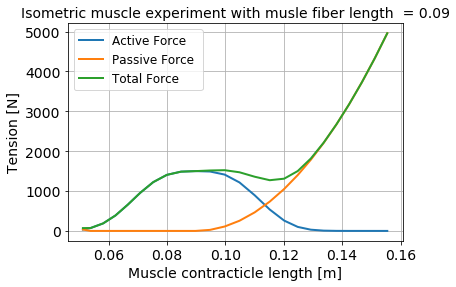
\includegraphics[height=0.3\columnwidth]{Lab5/Report/figures/1c_short.png}
  %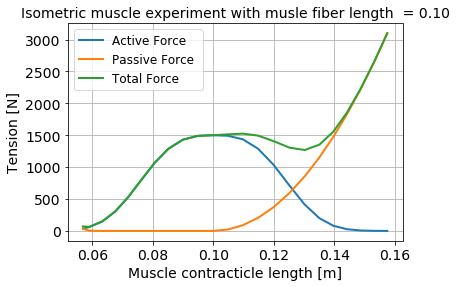
\includegraphics[height=0.3\columnwidth]{Lab5/Report/figures/1c_medium.png}
  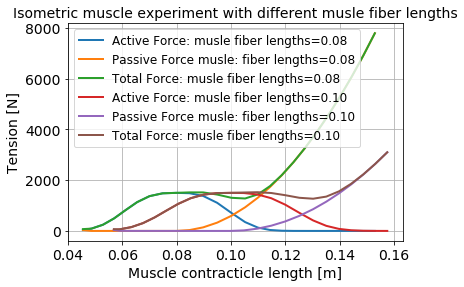
\includegraphics[height=0.4\columnwidth]{Lab5/Report/figures/1c.png}
  \caption{Relationship between forces and contractile element length with different muscle fiber lengths in isometric muscle experiment}
  \label{1c}
\end{figure}

No matter how the optimal length varies, the maximum active force obtained at that optimal length is always constant (as seen in the plots of Figure 6, where the maximum active force reaches 1500N in all cases). In addition, the obtained form of the plots does not change. As the maximum active force reached is dependent on the length of the muscle fiber, longer muscle fibers will require larger muscle stretch to reach this maximum active force value, and vice versa (longer muscle has larger compliance,meaning that when it is activated the slope of force-length is slightly lower). This also means that a larger fiber length means having a larger range of muscle contractile length, and vice versa. Furthermore,one need to pull the longer muscle more to activate the its resistance to stretch. 


\subsection*{Muscle Velocity-Tension Relationship}
In this exercise you will explore the relation between the force and
velocity of the muscle. In order to do this we replicate the set-up
show in figure \ref{fig:muscle-setup}. Here the length of the muscle
is allowed to vary by attaching one of its end to a fixed point and
the other to a variable external load. While applying a constant load
initially and holding the muscle at constant length, a quick release
is performed to let the muscle contract and pull the weight. The
maximum velocity during this quick release will give us the
relationship between muscle contractile velocity and the force.


\corr{Note} : Since the velocity changes sign and you need to compute the maximum
velocity accordingly by checking if the muscle was stretched or compressed
at the end of the experiment.

\begin{equation}
  \label{eq:2}
 V_{ce} = \left\{
\begin{array}{ll}
      min(v_{ce}(t)) & l_{mtu} < (l_{opt} + l_{slack}) \\
      max(v_{ce}(t)) & else \\
\end{array}
\right.
\end{equation}

\subsection*{1.d For a stimulation of 1.0 and starting at optimal
  muscle length, explore the relationship between contractile element
  velocity and external load. Plot the Velocity-Tension relationship
  curve. Include shortening and lengthening regions. Use the
  \fileref{isotonic\_muscle\_system.py::IsotonicMuscleSystem} instance
  to setup your experiment in \fileref{exercise1.py}}
  
  
\begin{figure}[H]
  \centering 
  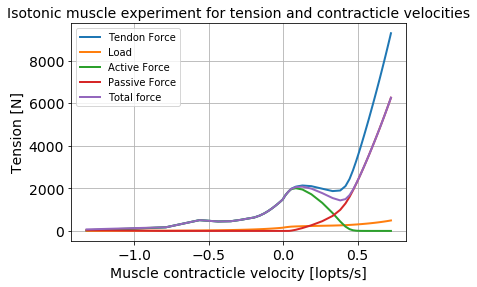
\includegraphics[height=0.3\columnwidth]{Lab5/Report/figures/1d.png}
  \caption{Relationship between muscle contractile velocity and tensions in isotonic muscle experiment}
  \label{1d}
\end{figure}

In the negative velocity range (contracting range), as the external load increases, the total force in the muscles increases. However, the main component of this total force is the active force, with the passive force being nearly zero. From Figure 5, it is seen that for a stimulation of 1.0, the muscle tension forces reach a maximum of 1500N for a given optimal muscle length. This value is in fact the value of the active force in the muscle. Back to Figure 7 above, as the velocity value increases in the negative range, the total force keeps on increasing until zero velocity is reached. This is the point with maximum contraction possible, and since stimulation is at 1.0, the force reached at zero velocity is 1500N. Beyond zero velocity, this is the lengthening range (positive velocity range). Here, the muscle is no longer able to support the load (the load is still increasing). Thus, the active force starts to decrease, and the passive force kicks in, resulting in a total force comprised mainly of the passive force values. Also, compared with the theory figures on lecture slides, plateau for high loads is missing. One possible reason may be approximation in computing the contractile velocity using min/max methods. 


\subsection*{1.e For the muscle force-velocity relationship, why is
  the lengthening force greater than the force output during
  shortening? No plots necessary}

As the muscle contracts (seen as an increase in velocity in the negative velocity range), the load is still supported. When reaching zero velocity, maximum muscle contraction is reached. Beyond this point (when lengthening starts), the active force decreases, and the passive force takes over. Since the passive force has the ability to continue increasing and reach higher values than the active force does, higher forces are achieved during lengthening. 

\subsection*{1.f What happens to the force-velocity relationship
  when the stimulation is varied between [0 - 1]? Support your
  response with one plot showing the different force-velocity
  relationship curves.  }

\begin{figure}[H]
  \centering 
  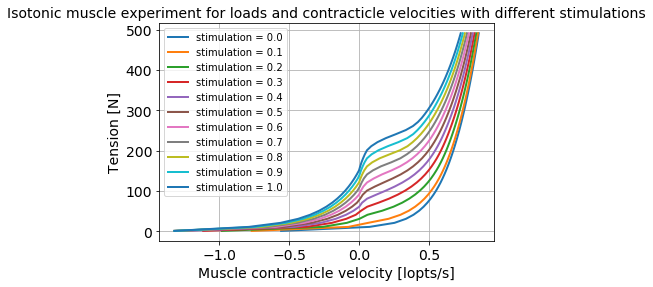
\includegraphics[height=0.3\columnwidth]{Lab5/Report/figures/1f_load.png}
  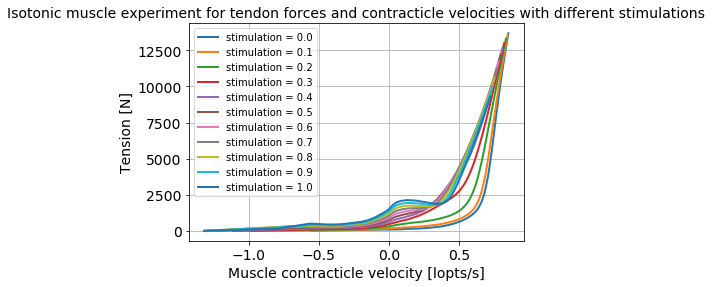
\includegraphics[height=0.3\columnwidth]{Lab5/Report/figures/1f_tendon.png}
  \caption{Relationship between muscle contractile velocity and tensions with different stimulations in isotonic muscle experiment}
  \label{1f}
\end{figure}

With increased stimulation, more muscle fiber units are activated. This is reflected as an increase in the load that can be supported by the muscle, as seen in Figure 8 above. In case of no stimulation, the muscle is not able to support the loads applied. In other words, it cannot contract, but rather stretch and lengthen. This is seen with blue curve (stimulation = 0.0) in the plots above, where this curve maintains a zero value in the negative velocity range (contraction range) to start increasing later on in the positive velocity range (lengthening range). This increase is mainly due to the existence of the passive force. Note that zero stimulation means there is an absence of the active force.  

\end{document}
